\section{\label{sec:level1}Measurement}

\begin{figure}[b]
\centering
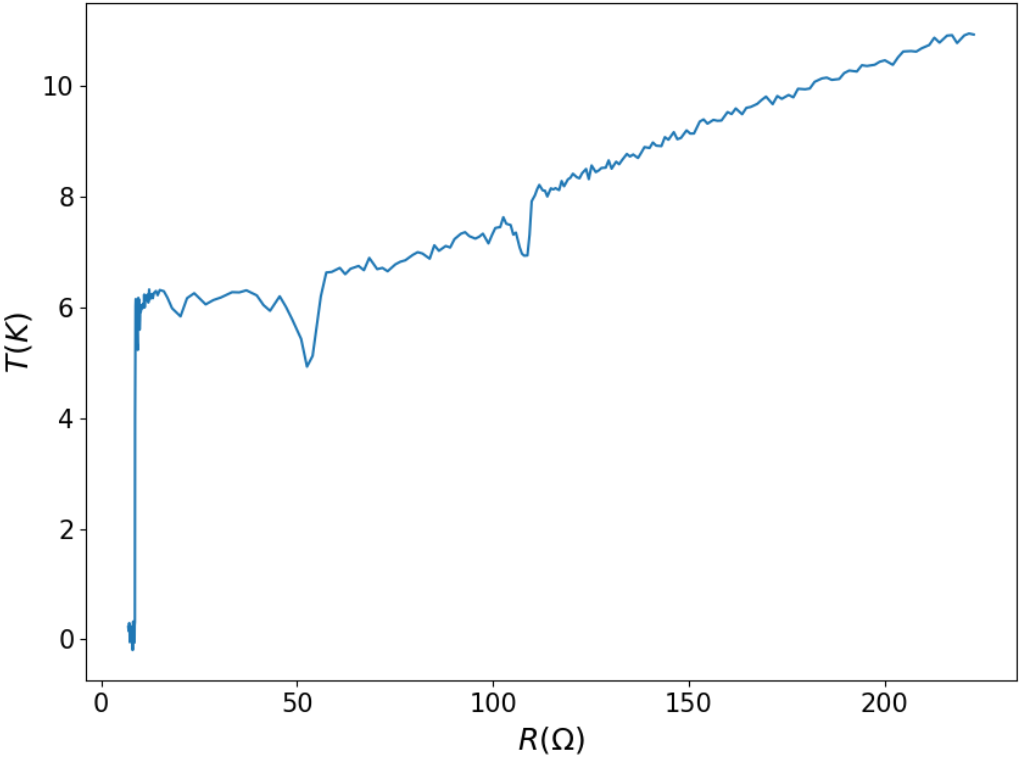
\includegraphics[height=0.275\textwidth,keepaspectratio]{RTPlot}
\caption{\label{fig:RTPlot}R-T plot for niobium where $T_C$$ = ($8.89 $\pm$ 0.01) K.}
\end{figure}

The SQUID electrical contact pads are wire bonded to a printed circuit board (PCB) in a four point connection. The combined sample is mounted within the inner vacuum chamber (IVC) of the cryostat where cooling processes using liquid ${}^4He$ reduces the sample temperature. Firstly the IVC is initially evacuated before a small amount of ${}^4He$ exchange gas enters the IVC by flushing the needle value and 1k pot valve to produce a $\approx$ 5 mbar pressure. Heat exchange with the 1 K pot reduces the temperature of the sample to $T_S$ $\approx$ 5 K. The thermal contact of the IVC and 1 K pot is removed. To achieve temperature cooling of $T_S$ $\approx$ 300 mK, ${}^3He$ must be condensation. The 1 K pot reaches a temperature below the boiling point of ${}^3He$, by liquid $^4He$ pumping, $^3He$ in contact with the 1 K pot is condensed $^[$\citep{HeManual}$^]$. Close cycle sorb pumping of $^3He$ through a charcoal sample in thermal contact with IVC is implemented and the sample reaches the base line temperature of $\approx$ 300 mK $^[$\citep{HeManual}$^]$. 

The initial dc measurement is completed during the cooling process by applying a small current source which flows through an uninterrupted section of $Nb$ film between the contact pads. The applied current ranges between $\pm$ 5 $\mu$A and the Voltage is measured.The resistance-temperature (R-T) plot is in Fig.(\ref{fig:RTPlot}) illustrates where the resistance drops to 0 and $Nb$ become superconducting at $T_C$ = (8.89 $\pm$ 0.01) K. The points at which the value of resistance appears to dip occurs when the cryostat probe is being lowered further into the liquid $4^He$ container.

\begin{figure}[t]
\centering
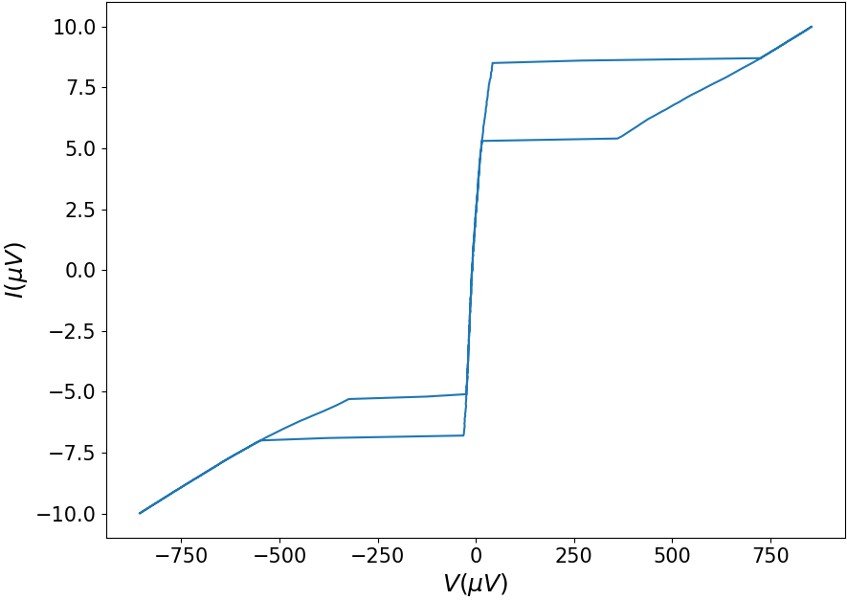
\includegraphics[height=0.275\textwidth,keepaspectratio]{IVplot}
\caption{\label{fig:IVplot}I-V curve for $B$ $\approx$ 0 mT. For positive current values $I_C$=(5.31 $\pm$0.05) $\mu$A, $I_{SW}$=(8.45 $\pm$0.05) $\mu$A. For negative current values $I_C$=-(5.30 $\pm$ 0.05) $\mu$A, $I_{SW}$=-(7.13 $\pm$0.05) $\mu$A}
\end{figure} 

The $I-V$ slope is measured by applying a dc current source to the SQUID in an applied $B$=0 field where $T_S\approx$ 0.3 K. The $I-V$ slope shown in Fig. (\ref{fig:IVplot}) exhibits a hysteric behaviour. This behaviour is expected to occur in weak-link JJs when $T_S$ is below 1.5 K $^[$\citep{Hao2015FabricationJunctions}$^]$. As the current is increased from 0 to 10 $\mu$A, the switching current $I_{SW}$=(8.45 $\pm$0.05) $\mu$A is the point at which the SQUID resistance becomes non-zero. The current source is then decreased to 0 and the critical current $I_C$=(5.31 $\pm$0.05) $\mu$A is observed as $Nb$ returns to being superconducting. The hysteric behaviour is believed to be due to current crowding through the JJs which results in heating of the device. This heating effect generates "hot spots" within the device when the current applied is > $I_{SW}$ $^[$\citep{Podd2007Micro-SQUIDsJunctions}$^]$. The asymmetry of the hysteresis for positive and negative source $I$ is related to the asymmetry of the left and right Dayem junction dimensions. The magnitude of the negative $I_{SW}$ is notably smaller than the positive $I_{SW}$. However the magnitude of $I_C$ does not change when the dc current is negative since $I_C$ is an bulk property of the $Ni$ SQUID.

The $I-V$ slope measurements are repeated throughout magnetic field sweeping of the SQUID in a range of $B$= $\pm$5 mT. For each $I-V$ data set there is 400 points which corresponds to the current increasing from 0 to 10 $\mu$A then decreasing to -10 $\mu$A and finally increasing to 0. The positive and negative $I_C$ values are obtained for each $I-V$ data set. The applied $B$ follows the same sequence of measurement as described for $I-V$ where the increment change in the applied field for each step is 0.04 mT. The temperature of the sample began increasing as the supply of ${}^4He$ ran out so the data for $B$ < 0 is disregarded.

\begin{figure}[b]
\centering
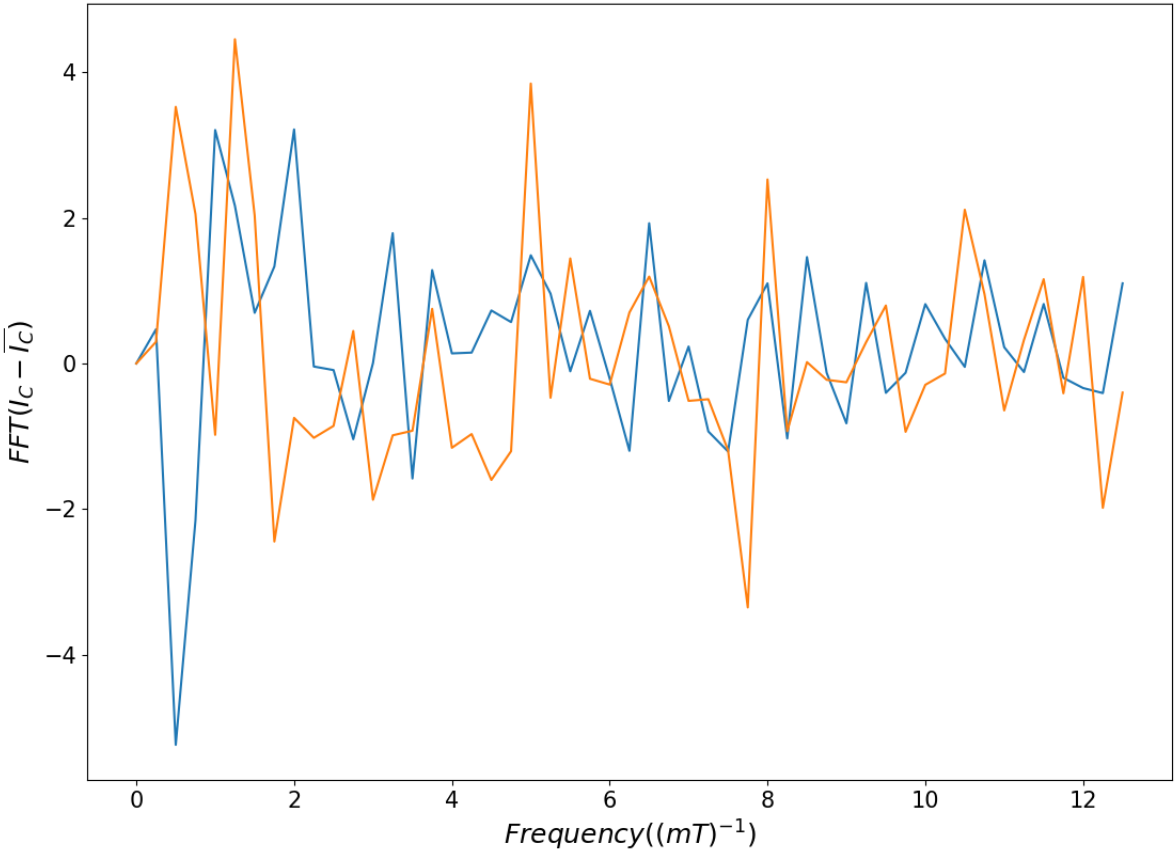
\includegraphics[height=0.275\textwidth,keepaspectratio]{ICbothB}
\caption{\label{fig:ICbothB}The FFT signal of the magnitude of the offset corrected positive (blue line) and negative (orange line) $I_C$ vs. $B$.}
\end{figure}

The range of $B$ is chosen as there is expected to be $\approx$9 periods of $\Phi _0$ for $B$ between 0 and 5 mT. However, there was no discernible periodic motion observed when plotting the positive and negative $I_C$ values against $B$. The Fast Fourier Transform (FFT) is applied to the magnitude of the offset corrected $I_C$ as shown in Fig. (\ref{fig:ICbothB}) when $B$ is increased from 0 to 5 mT. There are many frequency peaks observed in Fig. (\ref{fig:ICbothB}) which is expected to be due to the signal being noisy. However, a large peak is present for positive $I_C$ at a frequency of $\approx$ 0.5 (mT)\textsuperscript{-1}. This period corresponds to the calculated $B_0\approx$ 2 mT using Eq. \ref{eq:effectivearea} where $A_{eff}\approx$ $1 \times {10^{ - 12}}$ m. There is a peak also present at $\approx$ 0.5 (mT)\textsuperscript{-1} for negative $I_C$. However, the peak amplitude is not as large and there are other peaks at different frequency values with a similar amplitude. The FFT signal of the linear fit $R$ is is shown in Fig. (\ref{fig:RvsB}) where a large amplitude peak is also observed at $\approx$ 0.5 (mT)\textsuperscript{-1}. 

The FFT signal of $I_C$ and the FFT signal of linear fit of $R$ for $B$ decreasing towards 0 does not display a significantly large peak at $\approx$ 0.5 (mT)\textsuperscript{-1}. Therefore there is not sufficient evidence that the SQUID is oscillating sinusoidally at a particular frequency.

\begin{figure}[t]
\centering
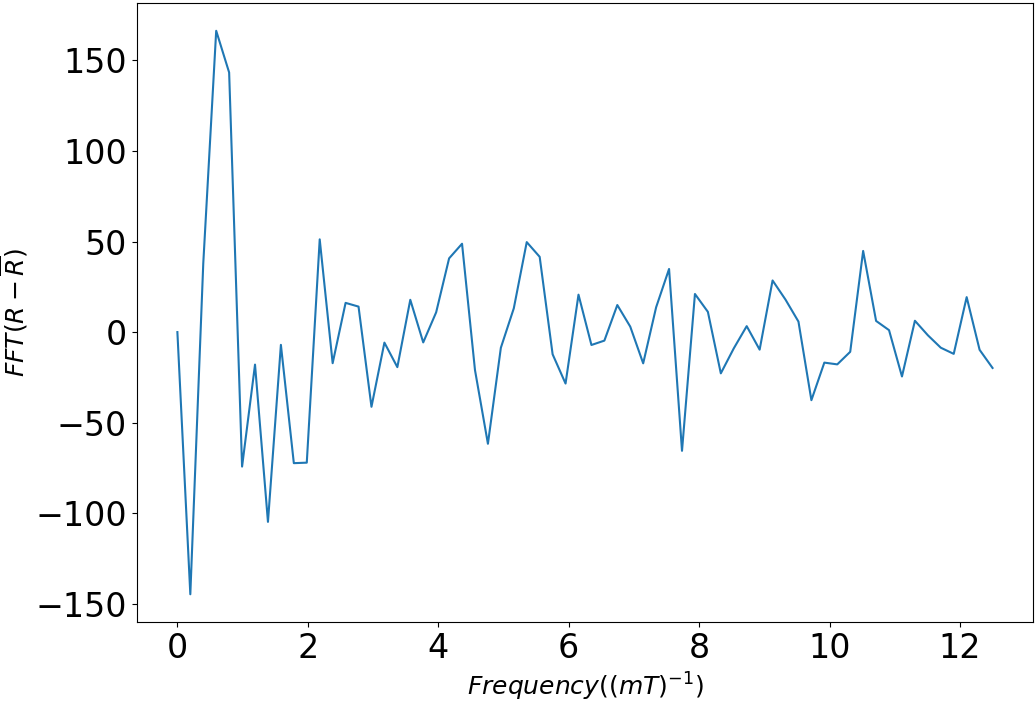
\includegraphics[height=0.275\textwidth,keepaspectratio]{RvsB}
\caption{\label{fig:RvsB}FFT signal of the linear fit resistance vs. $B$.}
\end{figure}

